\chapter{An optimization technique on pseudorandom generators based on chaotic iterations}
\minitoc
In this chapter, the statistical analysis of the three methods mentioned above are carried out systematically, and the results are discussed.
Indeed PRNGs are often based on modular arithmetic, logical operations like bitwise exclusive or (XOR), and on circular shifts of
bit vectors.
However the security level of some PRNGs of this kind has been revealed inadequate by today's standards.
Since different biased generators can possibly have their own side effects when inputted into our mixed generators, it is normal to enlarge the set of tested inputted PRNGs, to determine if the observed improvement still remains.
We will thus show in this research work that the intended statistical improvement is really effective for all of these most famous generators.



\section{About some Well-known PRNGs}
\label{The generation of pseudo-random sequence}

\subsection{Introduction}

Knowing that there is no universal generator, it is strongly recommended to test a stochastic application with a large set of different PRNGs~\cite{DavidRC2003643}. They can be classified in four major classes: linear generators, lagged generators, inversive generators, and mix generators:
\begin{itemize}
 \item \textbf{Linear generators}, defined by a linear recurrence, are the most commonly analyzed and utilized generators. The main linear generators are LCGs and MLCG.
 \item \textbf{Lagged generators} have a general recursive formula that use various previously computed terms in the determination of the new sequence value.
 \item \textbf{Inversive congruential generators} form a recent class of generators that are based on the principle of congruential inversion.
 \item \textbf{Mixed generators} result from the need for sequences of better and better quality, or at least longer periods. This has led to mix different types of PRNGs, as follows: $x^i=y^i\oplus z^i$
\end{itemize}


For instance, inversive generators are very interesting for verifying simulation results obtained with a linear congruential generator (LCG),
because their internal structure and correlation behavior strongly differs from what LCGs produce.
Since these generators have revealed several issues, some scientists refrain from using them.
In what follows, chaotic properties will be added to these PRNGs, leading to noticeable improvements observed by statistical test.
%Thus it helps scientists to enhance their habits by facilitating the use of sequences generated by generators that maybe they would not have used otherwise.
Let us firstly explain with more details the generators studied in this research work (for a synthetic view, see Fig.~\ref{Ontological class hierarchy of RNGs}).

\begin{figure}
\centering
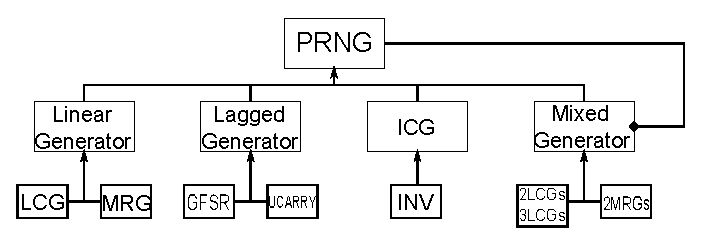
\includegraphics[width=3.5in]{TYPEPRNG.eps}
\DeclareGraphicsExtensions.
\caption{Ontological class hierarchy of PRNGs}
\label{Ontological class hierarchy of RNGs}
\end{figure}

\subsection{Details of some Existing Generators}

Here are the modules of PRNGs we have chosen to experiment.

\subsubsection{LCG}
This PRNG implements either the simple or the combined linear congruency generator (LCGs). The simple LCG is defined by the recurrence:
\begin{equation}
x^n = (ax^{n-1} + c)~mod~m
\label{LCG}
\end{equation}
where $a$, $c$, and $x^0$ must be, among other things, non-negative and less than $m$~\cite{Lecuyer2009}. In what follows, 2LCGs and 3LCGs refer as two (resp. three) combinations of such LCGs.
For further details, see~\cite{combined_lcg}.

\subsubsection{MRG}
This module implements multiple recursive generators (MRGs), based on a linear recurrence of order $k$, modulo $m$~\cite{Lecuyer2009}:
\begin{equation}
x^n = (a^1x^{n-1}+~...~+a^kx^{n-k})~mod~m
\label{MRG}
\end{equation}
Combination of two MRGs (referred as 2MRGs) is also be used in this paper.

\subsubsection{UCARRY}
Generators based on linear recurrences with carry are implemented in this module. This includes the add-with-carry (AWC) generator, based on the recurrence:
\begin{equation}
\label{AWC}
\begin{array}{l}
x^n = (x^{n-r} + x^{n-s} + c^{n-1})~mod~m, \\
c^n= (x^{n-r} + x^{n-s} + c^{n-1}) / m, \end{array}\end{equation}
the SWB generator, having the recurrence:
\begin{equation}
\label{SWB}
\begin{array}{l}
x^n = (x^{n-r} - x^{n-s} - c^{n-1})~mod~m, \\
c^n=\left\{
\begin{array}{l}
1 ~~~~~\text{if}~ (x^{i-r} - x^{i-s} - c^{i-1})<0\\
0 ~~~~~\text{else},\end{array} \right. \end{array}\end{equation}
%Implements the MWC generator:
%\begin{equation}
%\label{MWC}
%\begin{array}{l}
%x^n = (a^1x^{n-1} +~...~+a^rx^{n-r}+c^{n-1}) ~ mod ~ 2^w, \\
%c^n = (a^1x^{n-1} +~...~+a^rx^{n-r}+c^{n-1}) ~ /div ~ 2^w. \end{array}\end{equation}
and the SWC generator designed by R. Couture, which is based on the following recurrence:
\begin{equation}
\label{SWC}
\begin{array}{l}
x^n = (a^1x^{n-1} \oplus ~...~ \oplus a^rx^{n-r} \oplus c^{n-1}) ~ mod ~ 2^w, \\
c^n = (a^1x^{n-1} \oplus ~...~ \oplus a^rx^{n-r} \oplus c^{n-1}) ~ / ~ 2^w. \end{array}\end{equation}

\subsubsection{GFSR}
This module implements the generalized feedback shift register (GFSR) generator, that is:
\begin{equation}
x^n = x^{n-r} \oplus x^{n-k}
\label{GFSR}
\end{equation}

\subsubsection{INV}
Finally, this module implements the nonlinear inversive generator, as defined in~\cite{Lecuyer2009}, which is:

\begin{equation}
\label{INV}
\begin{array}{l}
x^n=\left\{
\begin{array}{ll}
(a^1 + a^2 / z^{n-1})~mod~m & \text{if}~ z^{n-1} \neq 0 \\
a^1 & \text{if}~  z^{n-1} = 0 .\end{array} \right. \end{array}\end{equation}


\section{statistical tests}
\label{Security analysis}

%A theoretical proof for the randomness of a generator is impossible to give, therefore statistical inference based on observed sample sequences produced by the generator seems to be the best option.
Considering the properties of binary random sequences, various statistical tests can be designed to evaluate the assertion that the sequence is generated by a perfectly random source. We have performed some statistical tests for the CIPRNGs proposed here. These tests include NIST suite~\cite{ANDREW2008} and DieHARD battery of tests~\cite{Marsaglia1996}. For completeness and for reference, we give in the following subsection a brief description of each of the aforementioned tests.

\subsection{NIST statistical tests suite}

Among the numerous standard tests for pseudo-randomness, a convincing way to show the randomness of the produced sequences is to confront them to the NIST (National Institute of  Standards and Technology) statistical tests, being an up-to-date tests suite proposed by the Information Technology Laboratory (ITL). A new version of the Statistical tests suite has been released in August 11, 2010.

The NIST tests suite SP 800-22 is a statistical package consisting of 15 tests. They were developed to test the randomness of binary sequences produced by hardware or software based cryptographic pseudorandom number generators. These tests focus on a variety of different types of non-randomness that could exist in a sequence.

For each statistical test, a set of $P-values$ (corresponding to the set of sequences) is produced.
The interpretation of empirical results can be conducted in various ways.
In this paper, the examination of the distribution of P-values to check for uniformity ($ P-value_{T}$) is used.
The distribution of $P-values$ is examined to ensure uniformity.
If $P-value_{T} \geqslant 0.0001$, then the sequences can be considered to be uniformly distributed.

In our experiments, 100 sequences (s = 100), each with 1,000,000-bit long, are generated and tested. If the $P-value_{T}$ of any test is smaller than 0.0001, the sequences are considered to be not good enough and the generating algorithm is not suitable for usage.





\subsection{DieHARD battery of tests}
The DieHARD battery of tests has been the most sophisticated standard for over a decade. Because of the stringent requirements in the DieHARD tests suite, a generator passing this battery of
tests can be considered good as a rule of thumb.

The DieHARD battery of tests consists of 18 different independent statistical tests. This collection
 of tests is based on assessing the randomness of bits comprising 32-bit integers obtained from
a random number generator. Each test requires $2^{23}$ 32-bit integers in order to run the full set
of tests. Most of the tests in DieHARD return a $P-value$, which should be uniform on $[0,1)$ if the input file
contains truly independent random bits.  These $P-values$ are obtained by
$P=F(X)$, where $F$ is the assumed distribution of the sample random variable $X$ (often normal).
But that assumed $F$ is just an asymptotic approximation, for which the fit will be worst
in the tails. Thus occasional $P-values$ near 0 or 1, such as 0.0012 or 0.9983, can occur.
An individual test is considered to be failed if the $P-value$ approaches 1 closely, for example $P>0.9999$.

\section{Results and discussion}
\label{Results and discussion}


\begin{sidewaystable}
\caption{NIST and DieHARD tests suite passing rates for PRNGs without CI}
\label{NIST and DieHARD tests suite passing rate the for PRNGs without CI}
\centering
\begin{tabular}{|l||c|c|c|c|c|c|c|c|c|c|}
    \hline\hline
Types of PRNGs & \multicolumn{2}{c|}{Linear PRNGs} & \multicolumn{4}{c|}{Lagged PRNGs} & \multicolumn{1}{c|}{ICG PRNGs} & \multicolumn{3}{c|}{Mixed PRNGs}\\ \hline
\backslashbox{\textbf{$Tests$}} {\textbf{$PRNG$}} & LCG& MRG& AWC & SWB  & SWC & GFSR & INV & LCG2& LCG3& MRG2 \\ \hline
NIST & 11/15 & 14/15 &\textbf{15/15} & \textbf{15/15}   & 14/15 & 14/15  & 14/15 & 14/15& 14/15& 14/15 \\ \hline
DieHARD & 16/18 & 16/18 & 15/18 & 16/18 & \textbf{18/18} & 16/18 & 16/18 & 16/18& 16/18& 16/18\\ \hline
\end{tabular}
\end{sidewaystable}



Table~\ref{NIST and DieHARD tests suite passing rate the for PRNGs without CI} shows the results on the batteries recalled above, indicating that almost all the PRNGs cannot pass all their tests. In other words, the statistical quality of these PRNGs cannot fulfill the up-to-date standards presented previously. We will show that the CIPRNG can solve this issue.

To illustrate the effects of this CIPRNG in detail, experiments will be divided in three parts:
\begin{enumerate}
  \item \textbf{Single CIPRNG}: The PRNGs involved in CI computing are of the same category.
  \item \textbf{Mixed CIPRNG}: Two different types of PRNGs are mixed during the chaotic iterations process.
  \item \textbf{Multiple CIPRNG}: The generator is obtained by repeating the composition of the iteration function as follows: $x^0\in \mathds{B}^{\mathsf{N}}$, and $\forall n\in \mathds{N}^{\ast },\forall i\in \llbracket1;\mathsf{N}\rrbracket,$
\begin{equation}
\begin{array}{l}
x_i^n=\left\{
\begin{array}{l}
x_i^{n-1}~~~~~\text{if}~S^n\neq i \\
\forall j\in \llbracket1;\mathsf{m}\rrbracket,f^m(x^{n-1})_{S^{nm+j}}~\text{if}~S^{nm+j}=i.\end{array} \right. \end{array}
\end{equation}
$m$ is called the \emph{functional power}.
\end{enumerate}


We have performed statistical analysis of each of the aforementioned CIPRNGs.
The results are reproduced in Tables~\ref{NIST and DieHARD tests suite passing rate the for PRNGs without CI} and \ref{NIST and DieHARD tests suite passing rate the for single CIPRNGs}.
The scores written in boldface indicate that all the tests have been passed successfully, whereas an asterisk ``*'' means that the considered passing rate has been improved.
\subsection{Tests based on the Single CIPRNG}

\begin{sidewaystable}
\renewcommand{\arraystretch}{1.3}
\caption{NIST and DieHARD tests suite passing rates for PRNGs with CI}
\label{NIST and DieHARD tests suite passing rate the for single CIPRNGs}
\centering
  \begin{tabular}{|l||c|c|c|c|c|c|c|c|c|c|c|c|}
    \hline
Types of PRNGs & \multicolumn{2}{c|}{Linear PRNGs} & \multicolumn{4}{c|}{Lagged PRNGs} & \multicolumn{1}{c|}{ICG PRNGs} & \multicolumn{3}{c|}{Mixed PRNGs}\\ \hline
\backslashbox{\textbf{$Tests$}} {\textbf{$Single~CIPRNG$}} & LCG  & MRG & AWC & SWB & SWC & GFSR & INV& LCG2 & LCG3& MRG2 \\ \hline\hline
Old CIPRNG\\ \hline \hline
NIST & \textbf{15/15} *  & \textbf{15/15} * & \textbf{15/15}   & \textbf{15/15}   & \textbf{15/15} * & \textbf{15/15} * & \textbf{15/15} *& \textbf{15/15} * & \textbf{15/15} * & \textbf{15/15} \\ \hline
DieHARD & \textbf{18/18} *  & \textbf{18/18} * & \textbf{18/18} *  & \textbf{18/18} *  & \textbf{18/18}  & \textbf{18/18} * & \textbf{18/18} *& \textbf{18/18} * & \textbf{18/18} *& \textbf{18/18} * \\ \hline
New CIPRNG\\ \hline \hline
NIST & \textbf{15/15} *  & \textbf{15/15} * & \textbf{15/15}   & \textbf{15/15}  & \textbf{15/15} * & \textbf{15/15} * & \textbf{15/15} *& \textbf{15/15} * & \textbf{15/15} * & \textbf{15/15} \\ \hline
DieHARD & \textbf{18/18} *  & \textbf{18/18} * & \textbf{18/18} * & \textbf{18/18} * & \textbf{18/18}  & \textbf{18/18} * & \textbf{18/18} * & \textbf{18/18} * & \textbf{18/18} *& \textbf{18/18} *\\ \hline
Xor CIPRNG\\ \hline\hline
NIST & 14/15*& \textbf{15/15} *   & \textbf{15/15}   & \textbf{15/15}   & 14/15 & \textbf{15/15} * & 14/15& \textbf{15/15} * & \textbf{15/15} *& \textbf{15/15}  \\ \hline
DieHARD & 16/18 & 16/18 & 17/18* & \textbf{18/18} * & \textbf{18/18}  & \textbf{18/18} * & 16/18 & 16/18 & 16/18& 16/18\\ \hline
\end{tabular}
\end{sidewaystable}

The statistical tests results of the PRNGs using the single CIPRNG method are given in Table~\ref{NIST and DieHARD tests suite passing rate the for single CIPRNGs}.
We can observe that, except for the Xor CIPRNG, all of the CIPRNGs have passed the 15 tests of the NIST battery and the 18 tests of the DieHARD one.
Moreover, considering these scores, we can deduce that both the single Old CIPRNG and the single New CIPRNG are relatively steadier than the single Xor CIPRNG approach, when applying them to different PRNGs.
However, the Xor CIPRNG is obviously the fastest approach to generate a CI random sequence, and it still improves the statistical properties relative to each generator taken alone, although the test values are not as good as desired.

Therefore, all of these three ways are interesting, for different reasons, in the production of pseudorandom numbers and,
on the whole, the single CIPRNG method can be considered to adapt to or improve all kinds of PRNGs.

To have a realization of the Xor CIPRNG that can pass all the tests embedded into the NIST battery, the Xor CIPRNG with multiple functional powers are investigated in Section~\ref{Tests based on Multiple CIPRNG}.



\subsection{Tests based on the Mixed CIPRNG}

To compare the previous approach with the CIPRNG design that uses a Mixed CIPRNG, we have taken into account the same inputted generators than in the previous section.
These inputted couples $(PRNG_1,PRNG_2)$ of PRNGs are used in the Mixed approach as follows:
\begin{equation}
\left\{
\begin{array}{l}
x^0 \in \llbracket 0, 2^\mathsf{N}-1 \rrbracket, S \in \llbracket 0, 2^\mathsf{N}-1 \rrbracket^\mathds{N} \\
\forall n \in \mathds{N}^*, x^n = x^{n-1} \oplus PRNG_1\oplus PRNG_2,
\end{array}
\right.
\label{equation Oplus}
\end{equation}

With this Mixed CIPRNG approach, both the Old CIPRNG and New CIPRNG continue to pass all the NIST and DieHARD suites.
In addition, we can see that the PRNGs using a Xor CIPRNG approach can pass more tests than previously.
The main reason of this success is that the Mixed Xor CIPRNG has a longer period.
Indeed, let $n_{P}$ be the period of a PRNG $P$, then the period deduced from the single Xor CIPRNG approach is obviously equal to:
\begin{equation}
n_{SXORCI}=
\left\{
\begin{array}{ll}
n_{P}&\text{if~}x^0=x^{n_{P}}\\
2n_{P}&\text{if~}x^0\neq x^{n_{P}}.\\
\end{array}
\right.
\label{equation Oplus}
\end{equation}

Let us now denote by $n_{P1}$ and $n_{P2}$ the periods of respectively the $PRNG_1$ and $PRNG_2$ generators, then the period of the Mixed Xor CIPRNG will be:
\begin{equation}
n_{XXORCI}=
\left\{
\begin{array}{ll}
LCM(n_{P1},n_{P2})&\text{if~}x^0=x^{LCM(n_{P1},n_{P2})}\\
2LCM(n_{P1},n_{P2})&\text{if~}x^0\neq x^{LCM(n_{P1},n_{P2})}.\\
\end{array}
\right.
\label{equation Oplus}
\end{equation}

In Table~\ref{DieHARD fail mixex CIPRNG}, we only show the results for the Mixed CIPRNGs that cannot pass all DieHARD suites (the NIST tests are all passed). It demonstrates that Mixed Xor CIPRNG involving LCG, MRG, LCG2, LCG3, MRG2, or INV cannot pass the two following tests, namely the ``Matrix Rank 32x32'' and the ``COUNT-THE-1's'' tests contained into the DieHARD battery. Let us recall their definitions:

\begin{itemize}
 \item \textbf{Matrix Rank 32x32.} A random 32x32 binary matrix is formed, each row having a 32-bit random vector. Its rank is an integer that ranges from 0 to 32. Ranks less than 29 must be rare, and their occurences must be pooled with those of rank 29. To achieve the test, ranks of 40,000 such random matrices are obtained, and a chisquare test is performed on counts for ranks 32,31,30 and for ranks $\leq29$.

 \item \textbf{COUNT-THE-1's TEST} Consider the file under test as a stream of bytes (four per  2 bit integer).  Each byte can contain from 0 to 8 1's, with probabilities 1,8,28,56,70,56,28,8,1 over 256.  Now let the stream of bytes provide a string of overlapping  5-letter words, each ``letter'' taking values A,B,C,D,E. The letters are determined by the number of 1's in a byte: 0,1, or 2 yield A, 3 yields B, 4 yields C, 5 yields D and 6,7, or 8 yield E. Thus we have a monkey at a typewriter hitting five keys with various probabilities (37,56,70,56,37 over 256).  There are $5^5$ possible 5-letter words, and from a string of 256,000 (over-lapping) 5-letter words, counts are made on the frequencies for each word.   The quadratic form in the weak inverse of the covariance matrix of the cell counts provides a chisquare test: Q5-Q4, the difference of the naive Pearson sums of $(OBS-EXP)^2/EXP$ on counts for 5- and 4-letter cell counts.
\end{itemize}

The reason of these fails is that the output of LCG, LCG2, LCG3, MRG, and MRG2 under the experiments are in 31-bit. Compare with the Single CIPRNG, using different PRNGs to build CIPRNG seems more efficient in improving random number quality (mixed Xor CI can 100\% pass NIST, but single cannot).

\begin{table*}
\renewcommand{\arraystretch}{1.3}
\caption{Scores of mixed Xor CIPRNGs when considering the DieHARD battery}
\label{DieHARD fail mixex CIPRNG}
\centering
  \begin{tabular}{|l||c|c|c|c|c|c|}
    \hline
\backslashbox{\textbf{$PRNG_1$}} {\textbf{$PRNG_0$}} & LCG & MRG & INV & LCG2 & LCG3 & MRG2 \\ \hline\hline
LCG  &\backslashbox{} {} &16/18&16/18 &16/18 &16/18 &16/18\\ \hline
MRG &16/18 &\backslashbox{} {} &16/18&16/18 &16/18  &16/18\\ \hline
INV &16/18 &16/18&\backslashbox{} {} &16/18 &16/18&16/18    \\ \hline
LCG2  &16/18 &16/18 &16/18 &\backslashbox{} {}  &16/18&16/18\\ \hline
LCG3  &16/18 &16/18 &16/18&16/18&\backslashbox{} {} &16/18\\ \hline
MRG2 &16/18  &16/18 &16/18&16/18 &16/18 &\backslashbox{} {}  \\ \hline
\end{tabular}
\end{table*}

\subsection{Tests based on the Multiple CIPRNG}
\label{Tests based on Multiple CIPRNG}

Until now, the combination of at most two input PRNGs has been investigated.
We now regard the possibility to use a larger number of generators to improve the statistics 
of the generated pseudorandom numbers, leading to the multiple functional power approach.
For the CIPRNGs which have already pass both the NIST and DieHARD suites with 2 inputted PRNGs 
(all the Old and New CIPRNGs, and some of the Xor CIPRNGs), it is not meaningful to consider 
their adaption of this multiple CIPRNG method, hence only the Multiple Xor CIPRNGs, 
having the following form, will be investigated.
\begin{equation}
\left\{
\begin{array}{l}
x^0 \in \llbracket 0, 2^\mathsf{N}-1 \rrbracket, S \in \llbracket 0, 2^\mathsf{N}-1 \rrbracket^\mathds{N} \\
\forall n \in \mathds{N}^*, x^n = x^{n-1} \oplus S^{nm}\oplus S^{nm+1}\ldots \oplus S^{nm+m-1} ,
\end{array}
\right.
\label{equation Oplus}
\end{equation}

The question is now to determine the value of the threshold $m$ (the functional power) making 
the multiple CIPRNG being able to pass the whole NIST battery.
Such a question is answered in Table~\ref{threshold}.


\begin{table*}
\renewcommand{\arraystretch}{1.3}
\caption{Functional power $m$ making it possible to pass the whole NIST battery}
\label{threshold}
\centering
  \begin{tabular}{|l||c|c|c|c|c|c|c|c|}
    \hline
Inputted $PRNG$ & LCG & MRG & SWC & GFSR & INV& LCG2 & LCG3  & MRG2 \\ \hline\hline
Threshold  value $m$& 19 & 7  & 2& 1 & 11& 9& 3& 4\\ \hline\hline
\end{tabular}
\end{table*}

\subsection{Results Summary}

We can summarize the obtained results as follows.
\begin{enumerate}
\item The CIPRNG method is able to improve the statistical properties of a large variety of PRNGs.
\item Using different PRNGs in the CIPRNG approach is better than considering several instances of one unique PRNG.
\item The statistical quality of the outputs increases with the functional power $m$.
\end{enumerate}

In this chapter, we first have formalized the CI methods that has been already presented in previous Internet conferences.
These CI methods are based on iterations that have been topologically proven as chaotic.
Then 10 usual PRNGs covering all kinds of generators have been applied, and the NIST and DieHARD batteries have been tested.
Analyses show that PRNGs using the CIPRNG methods do not only inherit the chaotic properties of the
CI iterations, they also have improvements of their statistics.
This is why CIPRNG techniques should be considered as post-treatments on pseudorandom number generators to improve both their randomness and security.

